\pagebreak
\section{Použitie webovej aplikácie}

\subsection{Registrácia}
Po otvorení aplikácie je nutné kliknúť na tlačidlo registrácie \textit{REGISTER}. Po vypnení údajov kliknúť na tlačidlo \textit{SUBMIT}.

\begin{figure}[H]
    \centering
    \begin{subfigure}{0.45\textwidth}
        \centering
        
\includegraphics[width=.7\textwidth]{guide_includes/img/register_button.png}
    \end{subfigure}
    \begin{subfigure}{0.45\textwidth}
        \centering
        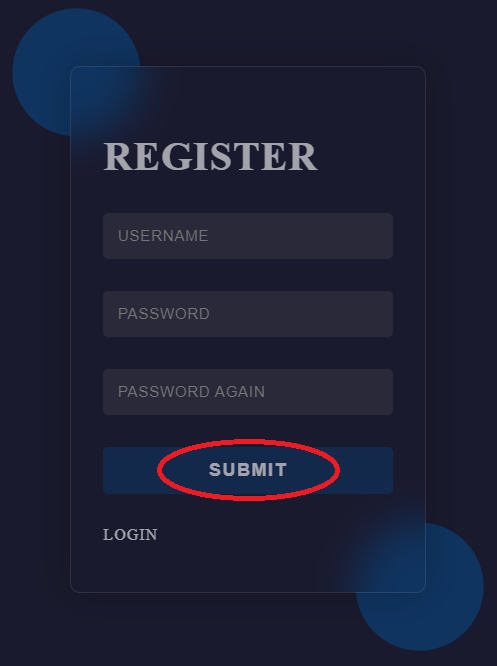
\includegraphics[width=.7\textwidth]{guide_includes/img/register_submit.png}
    \end{subfigure}
\end{figure}


\subsection{Prihlásenie}
Po otvorení aplikácie a vyplnení údajov kliknúť na tlačidlo \textit{SUBMIT}.
\begin{figure}[H]
    \centering
    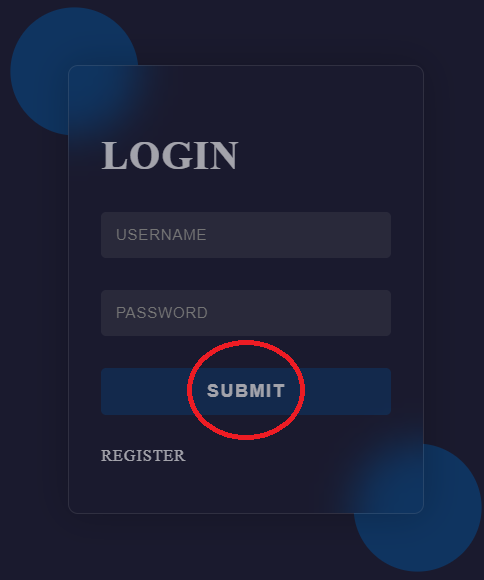
\includegraphics[width=0.3\textwidth]{guide_includes/img/login_submit.png}
\end{figure}


\subsection{Odhlásenie}
Pre odhlásenie kliknite na tlačidlo \textit{Profile} v pravej hornej časti mapy a následne kliknite na tlačidlo \textit{Logout}.
\begin{figure}[H]
    \centering
    \begin{subfigure}{0.45\textwidth}
        \centering
        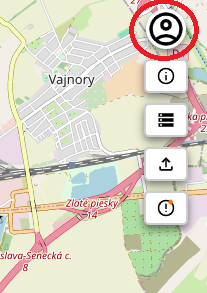
\includegraphics[width=.7\textwidth]{guide_includes/img/profile_button.png}
    \end{subfigure}
    \begin{subfigure}{0.45\textwidth}
        \centering
        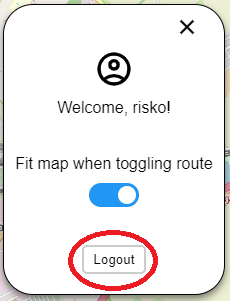
\includegraphics[width=.7\textwidth]{guide_includes/img/logout_button.png}
    \end{subfigure}
\end{figure}


\subsection{Nahranie trás}
Kliknite na tlačidlo \textit{Upload file} v pravej hornej časti mapy. Po otvorení okna zvoľte parametre pripínania trás k cestnej sieti. Po prejdení myšou ponad obrázok 
\includegraphics[scale=0.5]{img/icons/info.png} sa zobrazí vysvetlivka pre každý parameter. Pre výber ZIP súboru kliknite na tlačidlo \textit{Choose File} a vyberte súbor. Pre potvrdenie kliknite na tlačidlo \textit{Upload} a čakajte. Po skončení spracovania ZIP súboru uvidíte okno oznamujúce výsledok spracovania. 
\begin{figure}[H]
    \centering
    \begin{subfigure}{0.2\textwidth}
        \centering
        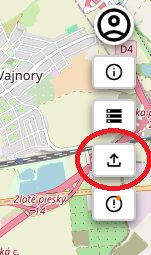
\includegraphics[width=1\textwidth]{guide_includes/img/upload_file_tool_button.png}
    \end{subfigure}
    \begin{subfigure}{0.78\textwidth}
        \centering
        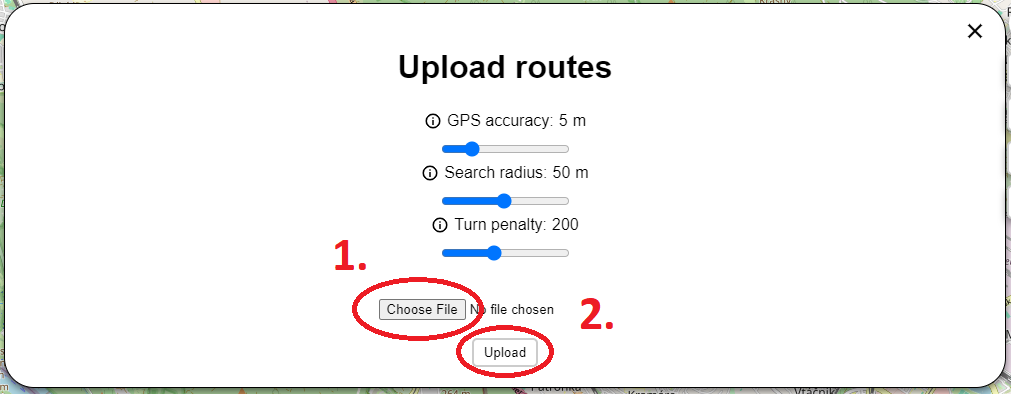
\includegraphics[width=1\textwidth]{guide_includes/img/upload_file.png}
    \end{subfigure}
\end{figure}


\subsection{Zobrazenie nahraných súborov\label{section:how_to_open_uploaded_files}}
Kliknite na tlačidlo \textit{Show Files}. Otvorí sa okno, ktoré v tabuľke zobrazuje nahrané súbory spolu s dátumom nahrania a prepínačmi pre zobrazenie trás na mape.
\begin{figure}[H]
    \centering
    \begin{subfigure}{0.2\textwidth}
        \centering
        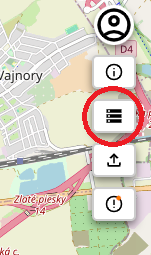
\includegraphics[width=1\textwidth]{guide_includes/img/show_files_tool_button.png}
    \end{subfigure}
    \begin{subfigure}{0.78\textwidth}
        \centering
        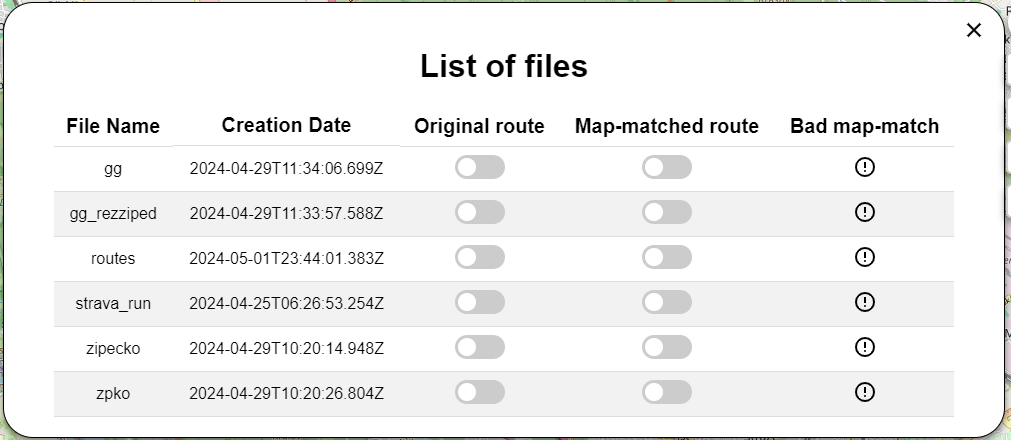
\includegraphics[width=1\textwidth]{guide_includes/img/uploaded_files_window.png}
    \end{subfigure}
\end{figure}

\subsection{Zobrazenie všetkyćh trás v nahranom súbore}
Otvorte okno s nahratými súbormi podľa návodu v sekcií \ref{section:how_to_open_uploaded_files}. Po otvorení okna kliknite na prepínač. 
\begin{figure}[H]
    \centering
    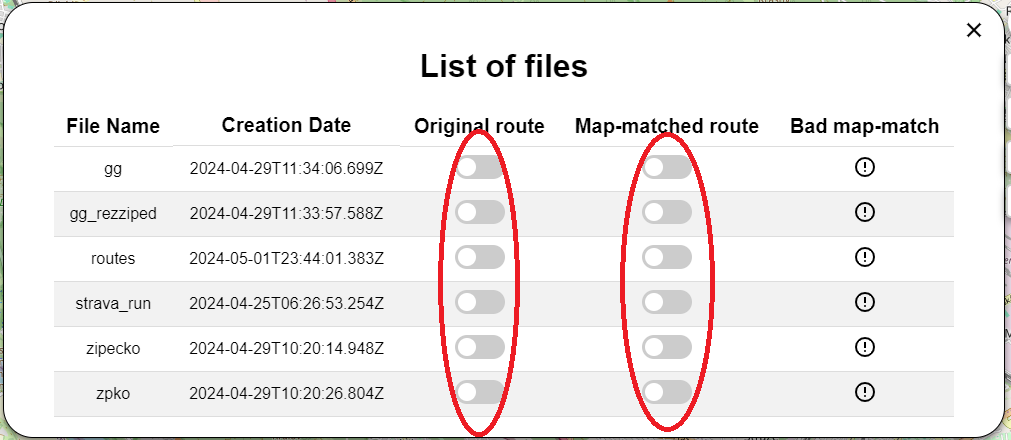
\includegraphics[width=1\textwidth]{guide_includes/img/toggle_all_routes.png}
\end{figure}

\pagebreak
\subsection{Zobrazenie jednotlivých trás v nahranom súbore}
Otvorte okno s nahratými súbormi podľa návodu v sekcií \ref{section:how_to_open_uploaded_files}. Po otvorení okna kliknite na názov súboru, ktorého trasy chcete zobraziť. Po otvorení okna so zoznamom trás, ktoré zvolený súbor obsahuje kliknite na prepínač. 
\begin{figure}[H]
    \centering
    \begin{subfigure}{1\textwidth}
        \centering
        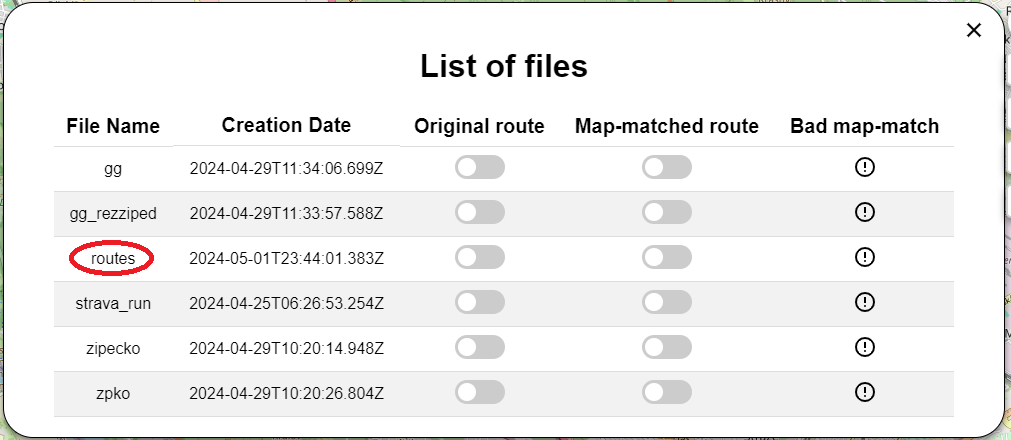
\includegraphics[width=1\textwidth]{guide_includes/img/open_file.png}
    \end{subfigure}
    \begin{subfigure}{1\textwidth}
        \centering
        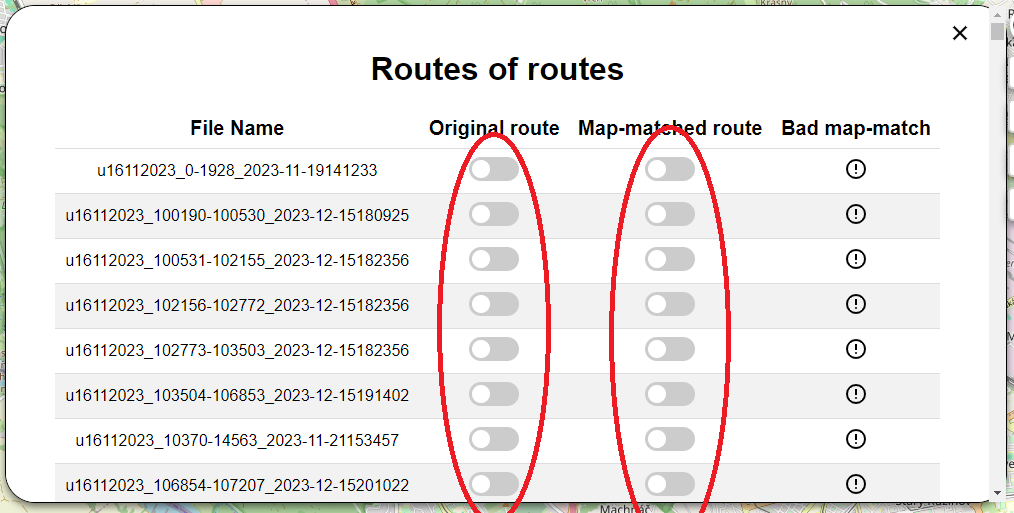
\includegraphics[width=1\textwidth]{guide_includes/img/toggle_route.png}
    \end{subfigure}
\end{figure}

\subsection{Zobrazenie chybových nahraných súborov\label{section:how_to_open_error_files}}
Kliknite na tlačidlo \textit{Error files} v pravej hornej časti mapy. Otvorí sa okno zobrazujúce chybové súbory v tabuľke.
\begin{figure}[H]
    \centering
    \begin{subfigure}{0.2\textwidth}
        \centering
        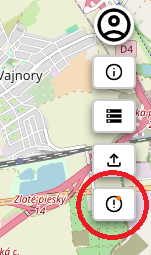
\includegraphics[width=1\textwidth]{guide_includes/img/show_errors_tool_button.png}
    \end{subfigure}
    \begin{subfigure}{.78\textwidth}
        \centering
        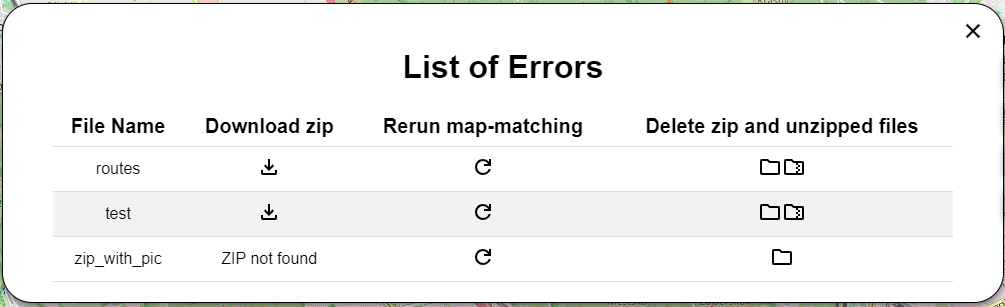
\includegraphics[width=1\textwidth]{guide_includes/img/errors.png}
    \end{subfigure}
\end{figure}

\subsection{Znovu-spustenie chybových súborov}
Otvorte okno s chybovými súbormi podľa návodu v sekcií \ref{section:how_to_open_error_files}. Kliknite na tlačidlo znovu-spustenia. V prípade, že sa nahraný ZIP súbor nepodarilo rozbaliť tlačidlo nebude zobrazené. 
\begin{figure}[H]
    \centering
    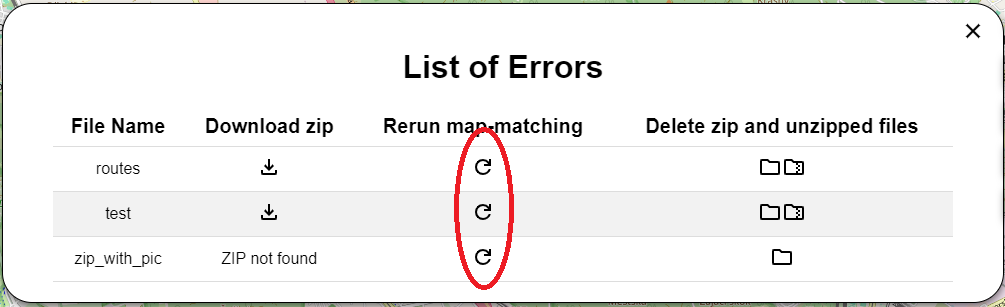
\includegraphics[width=1\textwidth]{guide_includes/img/rerun_map_match.png}
\end{figure}

\pagebreak
\subsection{Upozornenie na zlé pripnutie trasy k cestnej sieti}
Otvorte okno s nahratými súbormi podľa návodu v sekcií \ref{section:how_to_open_uploaded_files}. Po otvorení okna kliknite na tlačidlo upozornenia. 
\begin{figure}[H]
    \centering
    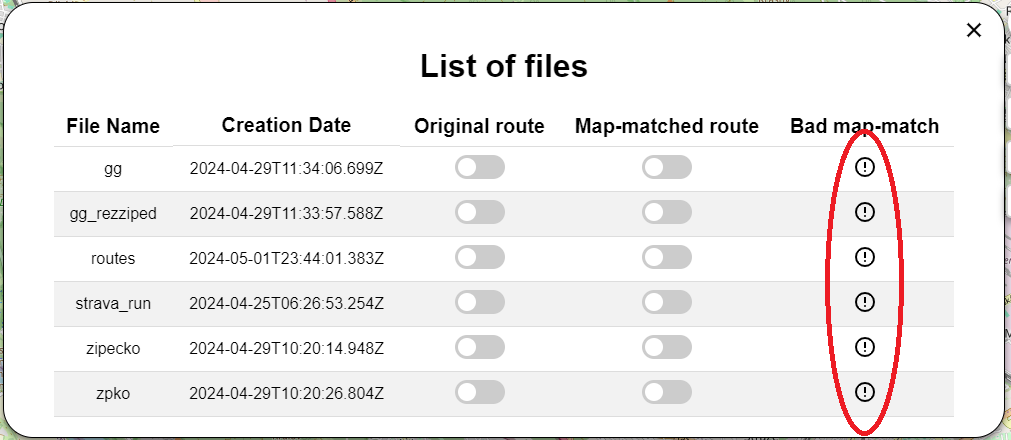
\includegraphics[width=1\textwidth]{guide_includes/img/bad_map_match_notify.png}
\end{figure}